% Slides for 2024-07-16
% To create a slide, use the following:
% \begin{frame}{TITLE}
%     BODY
% \end{frame}

% To create a slide with a bullet list, use the following:
% \begin{frame}{TITLE}
%     \begin{itemize}
%         \item ITEM 1
%         \item ITEM 2
%     \end{itemize}    
% \end{frame}

% To create a slide with numbered list, use the following:
% \begin{frame}{TITLE}
%     \begin{enumerate}
%         \item ITEM 1
%         \item ITEM 2
%     \end{enumerate}
% \end{frame}

% To create a slide with a graphic:
% 1. Add the graphic to this folder (named picture.png)
% 2. Use the following:
% \begin{frame}{TITLE}
%     \centering
%     \includegraphics[height=0.7\textheight,width=0.7\textwidth,keepaspectratio]{picture.png}
% \end{frame}

% To create a slide with two columns, use the following:
% \begin{frame}{TITLE}
%     \begin{columns}
%         \begin{column}{0.5\textwidth}
%             COLUMN 1 BODY
%         \end{column}
%         \begin{column}{0.5\textwidth}
%             COLUMN 2 BODY
%         \end{column}
%     \end{columns}
% \end{frame}

\begin{frame}{Remember from Two Weeks Ago}
    \begin{center}
        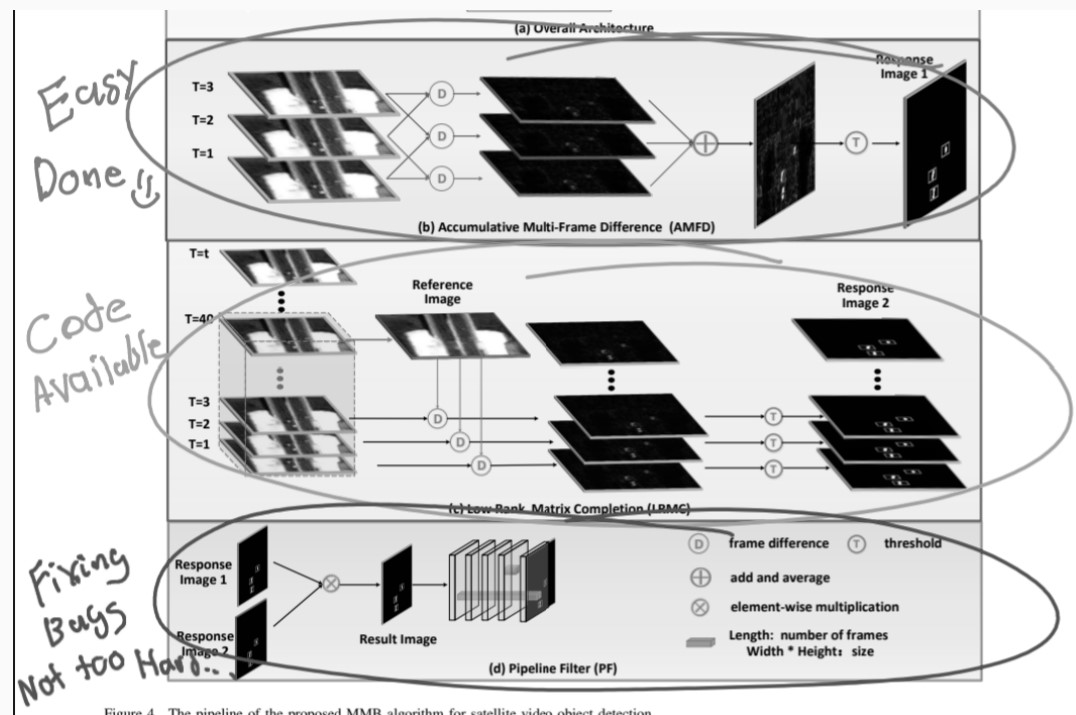
\includegraphics[height=0.7\textheight,width=0.7\textwidth,keepaspectratio]{images/baboon/old.jpg}
    \end{center}
    \begin{itemize}
        \item Solving solution stack.
    \end{itemize}
\end{frame}

\begin{frame}{Code deployment process}
    \begin{center}
        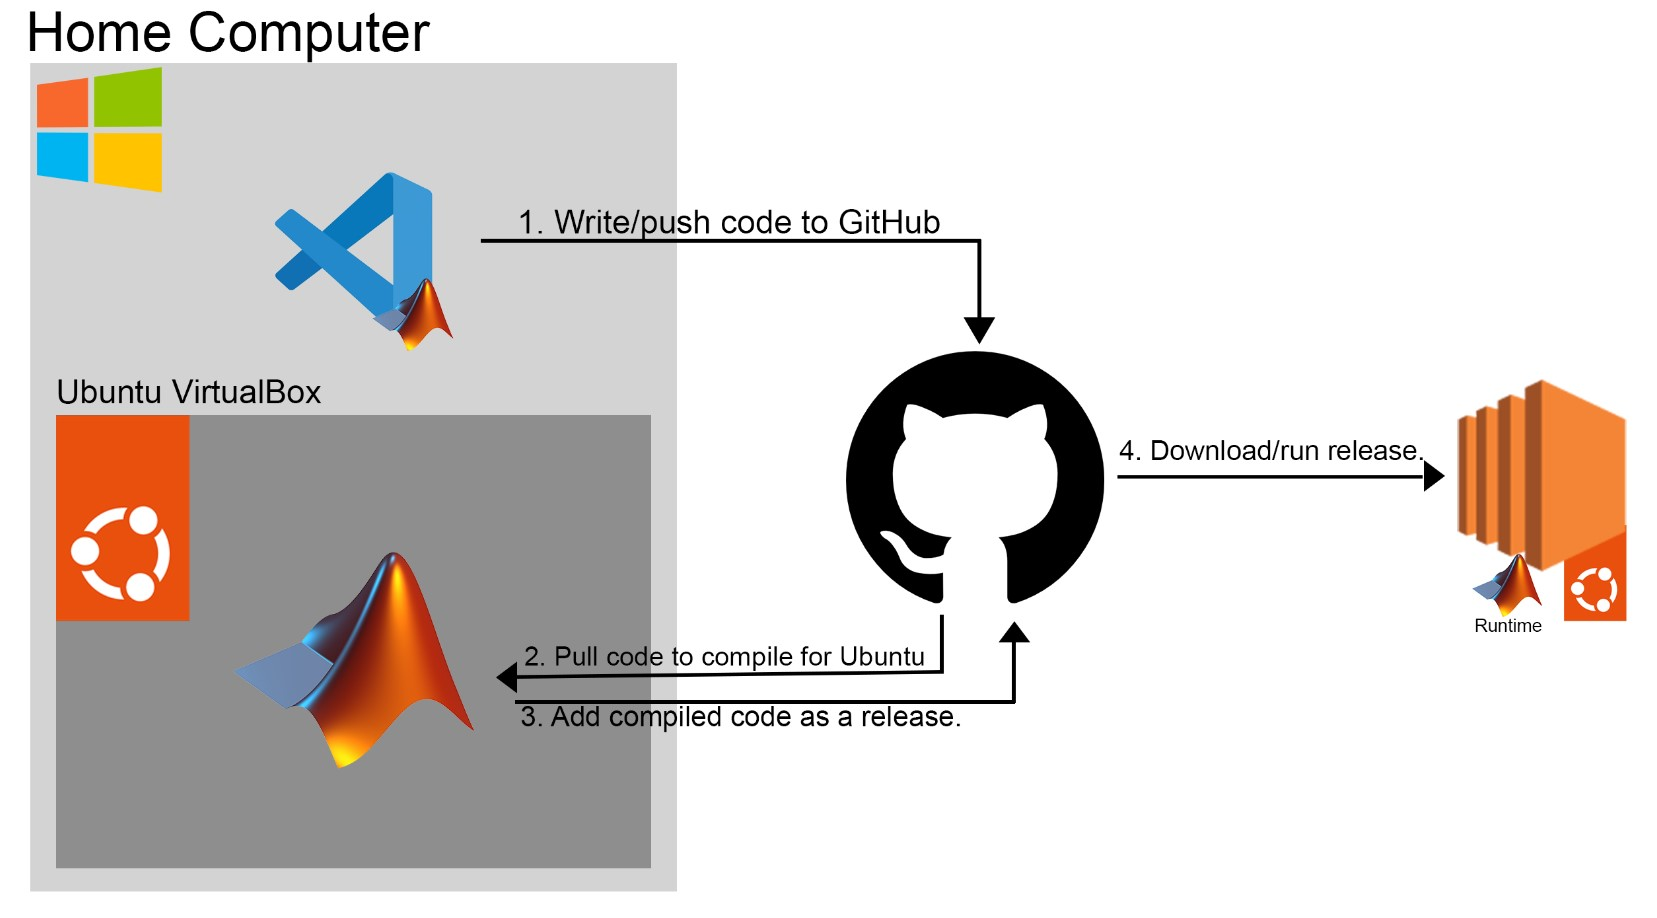
\includegraphics[height=0.7\textheight,width=0.7\textwidth,keepaspectratio]{images/baboon/Process.jpg}
    \end{center}
\end{frame}

\begin{frame}{Code optimization additions}
    \begin{itemize}
        \item Parallelization. (2-3 hours to 10-15 minutes)
        \item Stop earlies.
    \end{itemize}
\end{frame}

\begin{frame}{Scoring confusion.}
    \begin{center}
        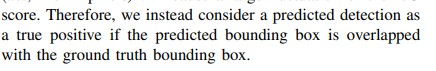
\includegraphics[height=0.7\textheight,width=0.7\textwidth,keepaspectratio]{images/baboon/text.jpg}
        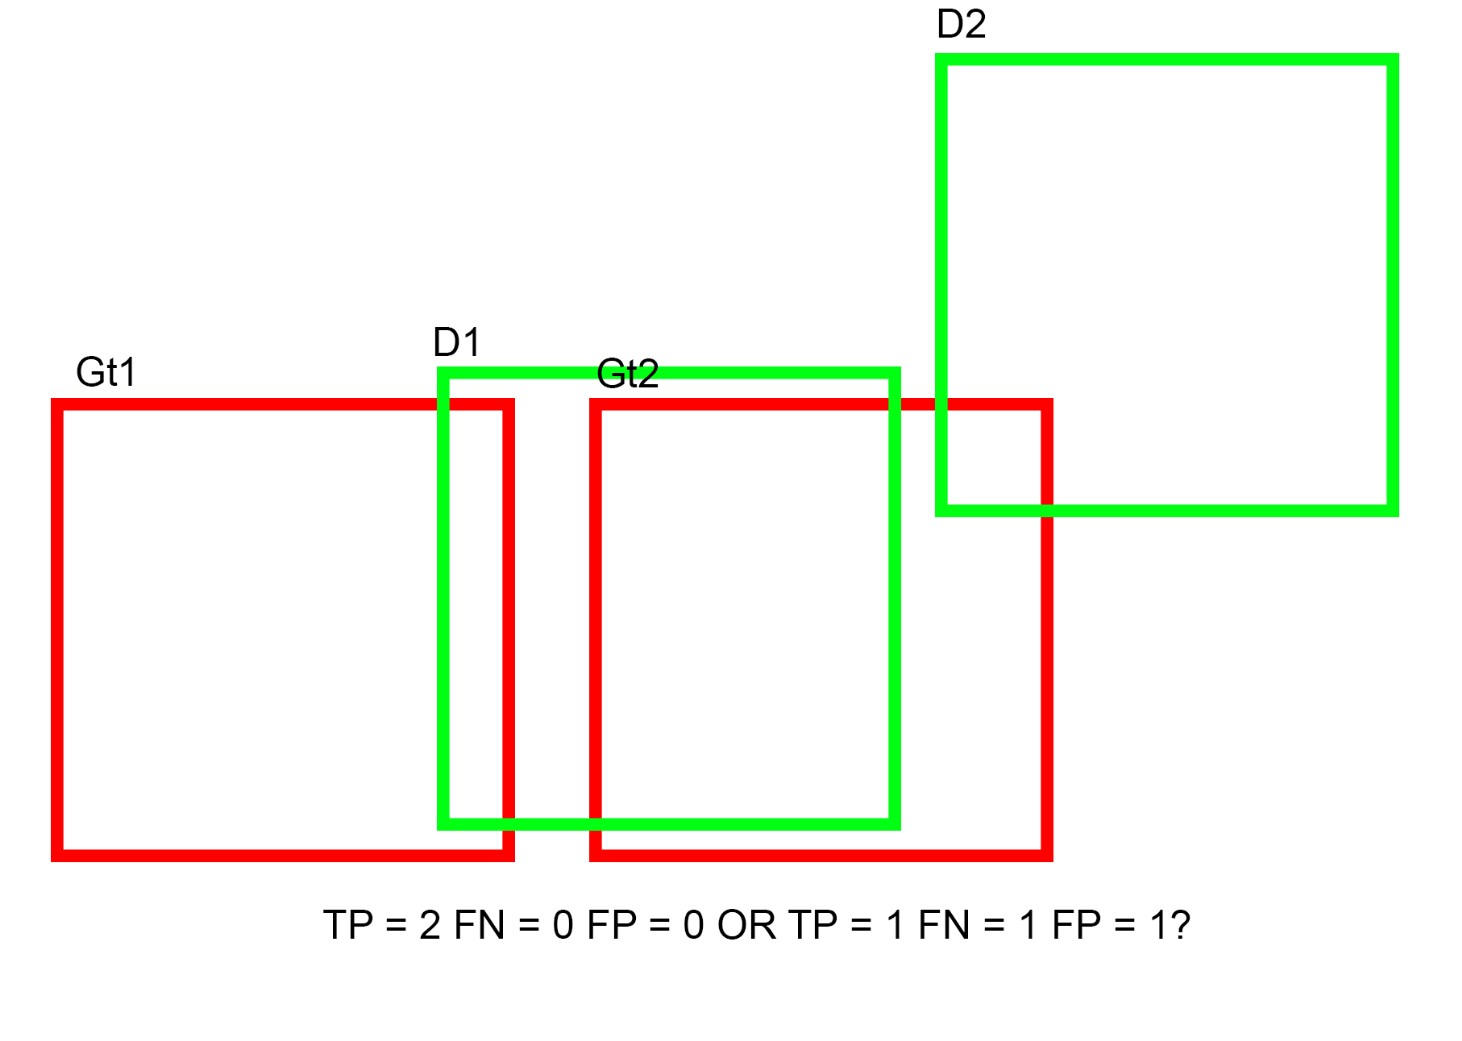
\includegraphics[height=0.7\textheight,width=0.7\textwidth,keepaspectratio]{images/baboon/gtd.jpg}
    \end{center}
\end{frame}

\begin{frame}{What next?}
    \begin{itemize}
        \item Pareto frontier optimization running right now.
        \item Will hopefully have results by next week.
        \item Getting ready to deploy SPOT again.
    \end{itemize}
\end{frame}